\documentclass[12pt]{article}
\usepackage[utf8]{inputenc}
\usepackage{graphicx} % Allows you to insert figures
\usepackage{amsmath} % Allows you to do equations
\usepackage{fancyhdr} % Formats the header
\usepackage{geometry} % Formats the paper size, orientation, and margins
\usepackage[style=authoryear-ibid,backend=biber]{biblatex} % Allows you to do citations - does Harvard style and compatible with Zotero
\addbibresource{Example.bib} % Tells LaTeX where the citations are coming from. This is imported from Zotero
\usepackage[english]{babel}
\usepackage{csquotes}
\usepackage{background}
\usepackage{minted}
\renewcommand*{\nameyeardelim}{\addcomma\space} % Adds comma in in-text citations
\linespread{1.5} % About 1.5 spacing in Word
\setlength{\parindent}{0pt} % No paragraph indents
\setlength{\parskip}{1em} % Paragraphs separated by one line
\renewcommand{\headrulewidth}{0pt} % Removes line in header
\geometry{a4paper, portrait, margin=1in}
\setlength{\headheight}{14.49998pt}
\backgroundsetup{scale=1,angle=0,opacity=0.175,contents={
\includegraphics[scale=0.25]{1200px-Vellore_Institute_of_Technology_seal_2017.png}}}


\begin{document}
\begin{titlepage}
\NoBgThispage
   \begin{center}
        \begin{figure}[h] % h - Place the float here, i.e., approximately at the same point it occurs in the source text (however, not exactly at the spot)
        \centering
        
\includegraphics[width=15cm]{1583124354phpJTtnK5.png}
        \end{figure}

        \Huge{Lab CAT 1}

        \vspace{0.5cm}
        \LARGE{20BIT0406 - Sanchit Sandeep Khedkar}
       
        \vspace{2.5 cm}
        \Large{2022-03-02}
        
        \vspace{0.25 cm}
        \Large{ITE2002 - Operating Systems}
        \large{VL2021220500441 L45+L46}
       

       \vfill
    \end{center}
\end{titlepage}
\newpage

\setcounter{page}{2}
\pagestyle{fancy}
\fancyhf{}
\rhead{\thepage}
Q. Create a process using fork() .Assign sorting of five numbers task to child process. Check given number is prime or not in parent process  (Use execl or execvp system call)
\\ \\ Ans-
\\ pgm.1.c -
\begin{figure}[h] % h - Place the float here, i.e., approximately at the same point it occurs in the source text (however, not exactly at the spot)
\centering
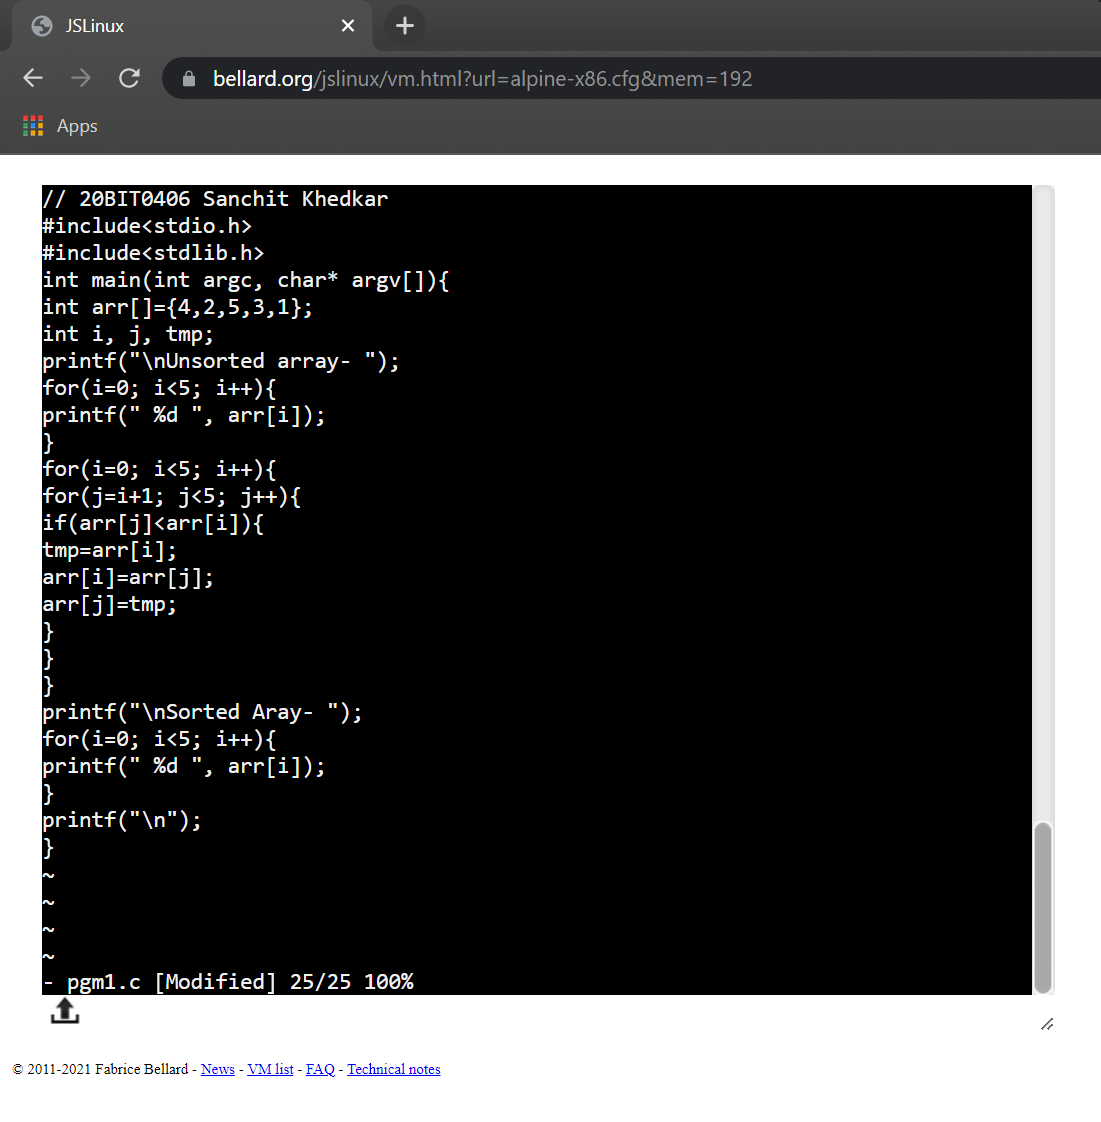
\includegraphics[width=\textwidth]{pgm1.png}
\caption{pgm1.c}
\end{figure}
\newpage
pgm2.c -
\begin{figure}[h] % h - Place the float here, i.e., approximately at the same point it occurs in the source text (however, not exactly at the spot)
\centering
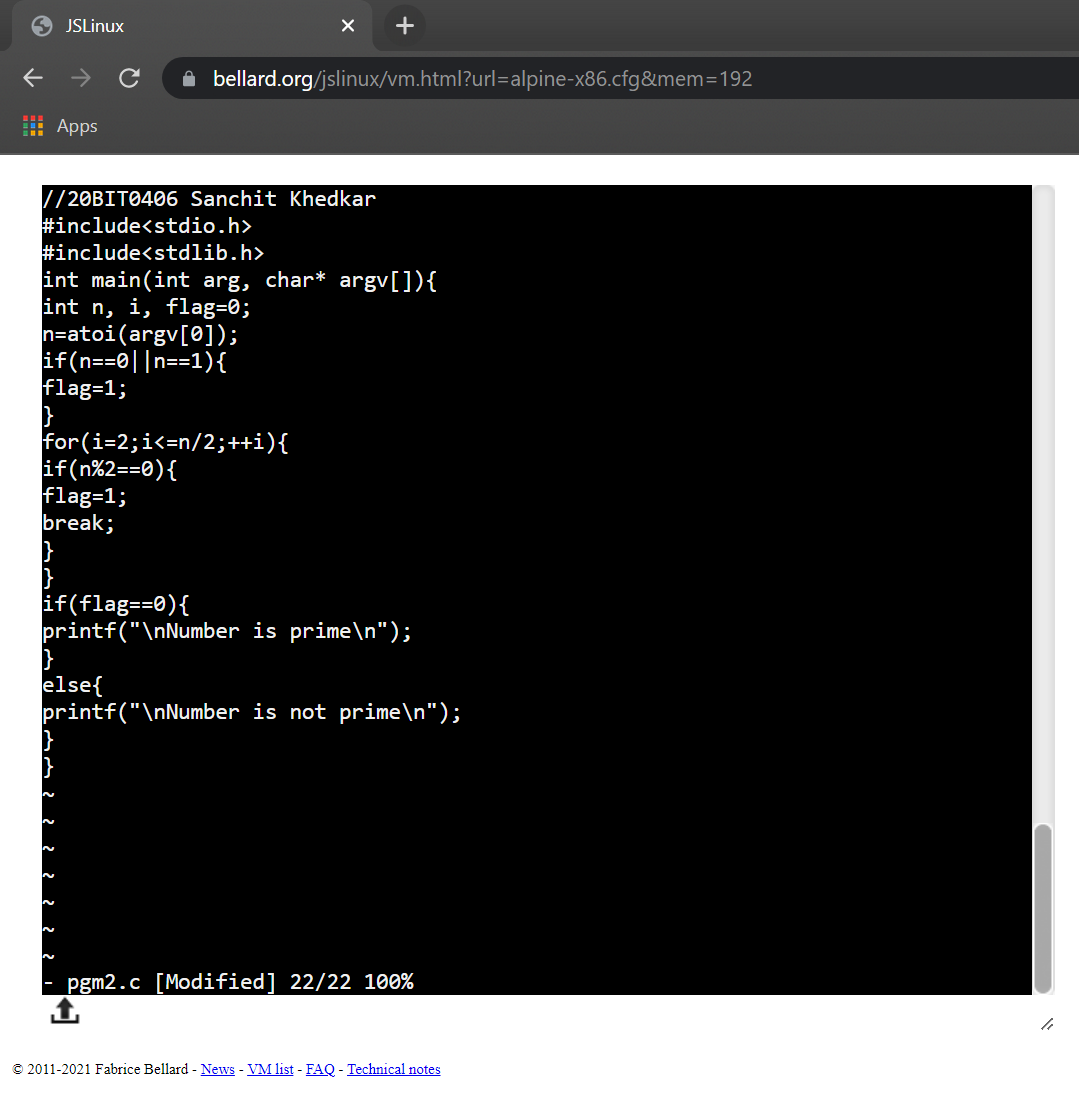
\includegraphics[width=\textwidth]{pgm2.png}
\caption{pgm2.c}
\end{figure}
\newpage
pgm3.c -
\begin{figure}[h] % h - Place the float here, i.e., approximately at the same point it occurs in the source text (however, not exactly at the spot)
\centering
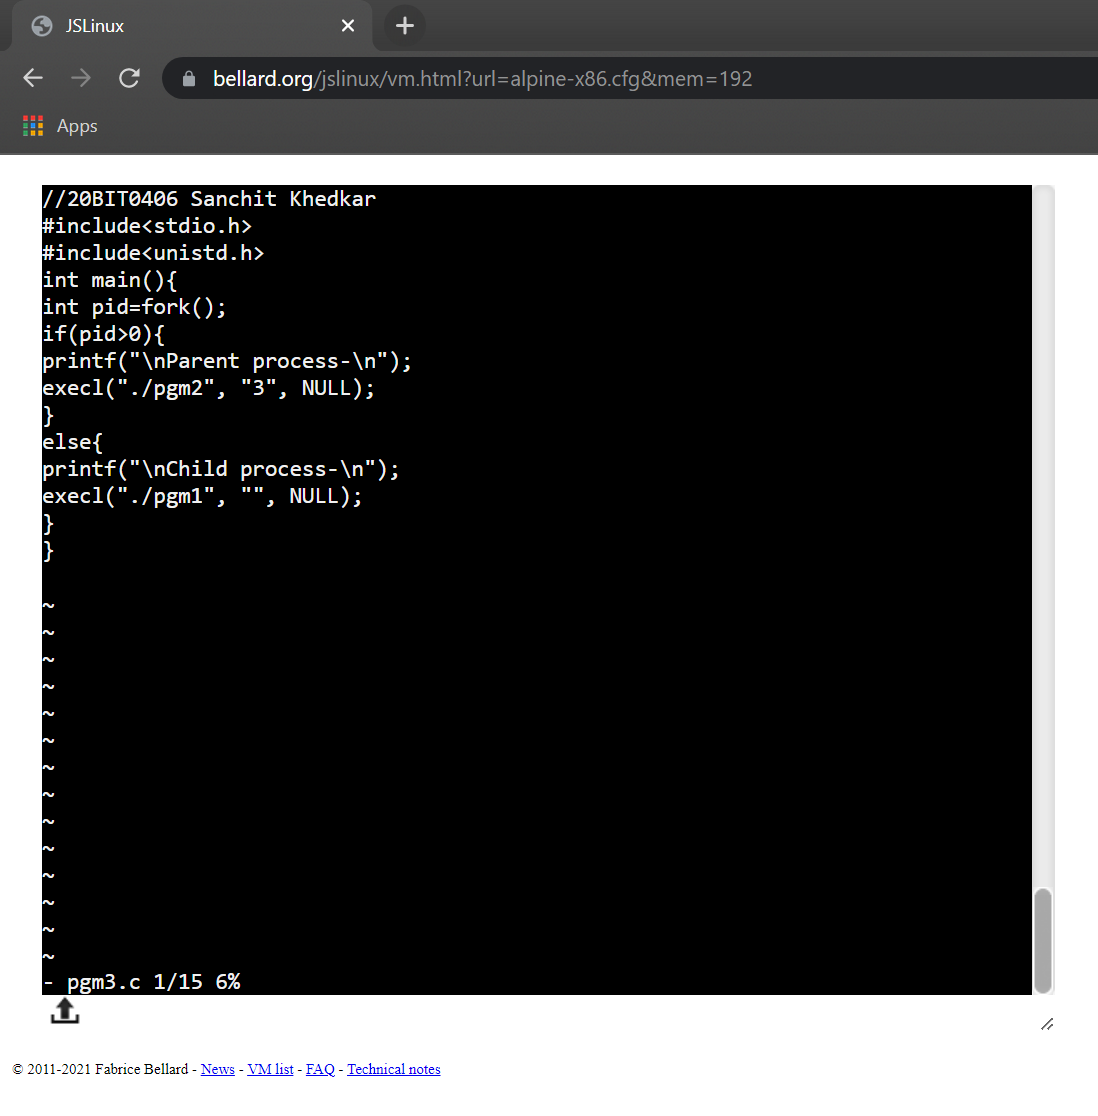
\includegraphics[width=\textwidth]{pgm3.png}
\caption{pgm3.c}
\end{figure}
\newpage
Output -
\begin{figure}[h] % h - Place the float here, i.e., approximately at the same point it occurs in the source text (however, not exactly at the spot)
\centering
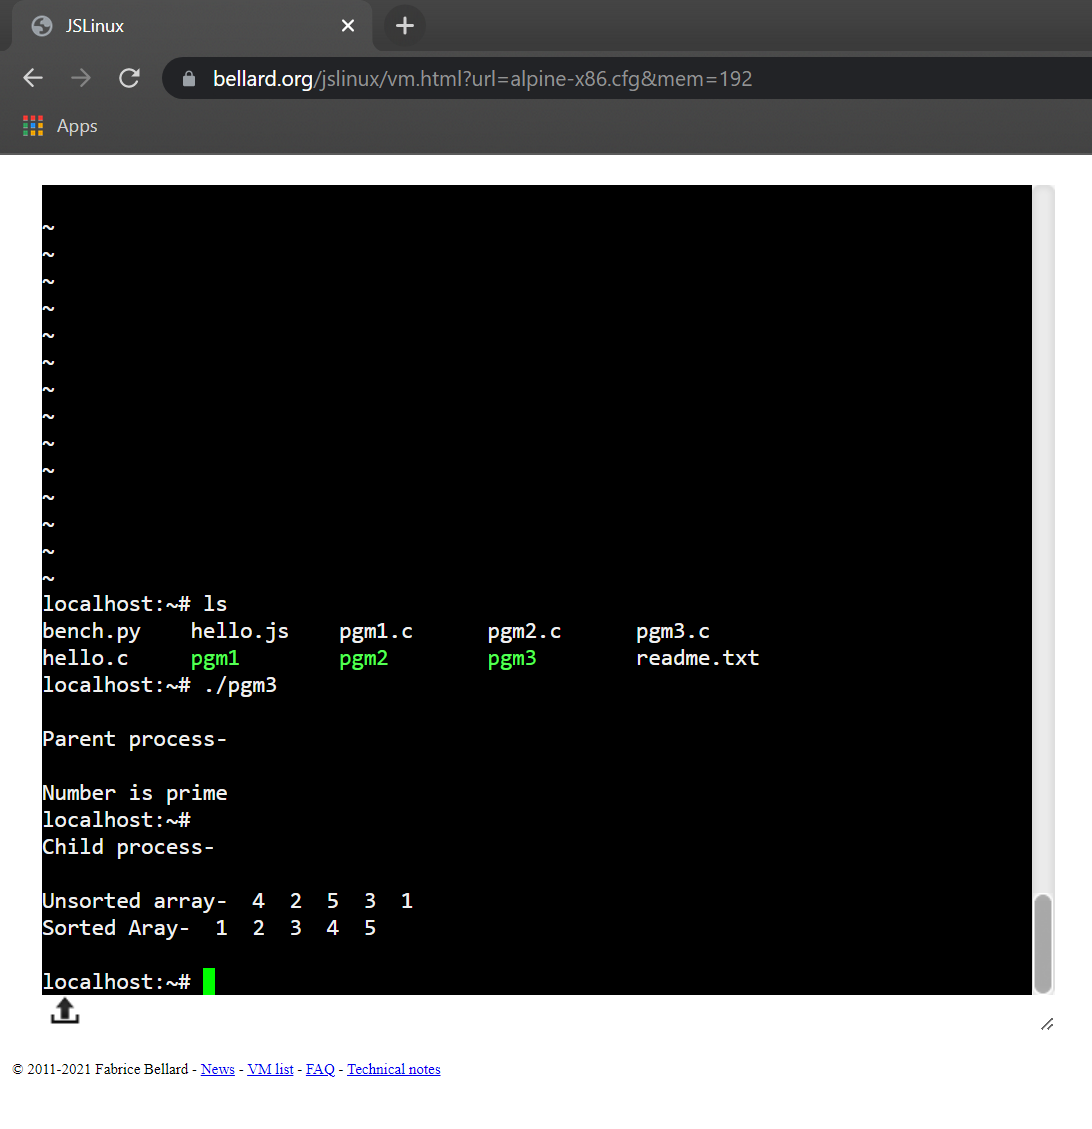
\includegraphics[width=\textwidth]{pgmoutput.png}
\caption{Ouptut}
\end{figure}
\end{document}
